\chapter{How it works}
\label{cha:How it works}
All concepts described in this chapter are referred by \cite{AmazonWebServices2013}.

\section{Core Components}
In DynamoDB, tables, items and attributes are the core components to work with. A table is a collection of items, and each item is a collection of attributes. 
These core components are very similar to other database systems.

\begin{figure}
\centering
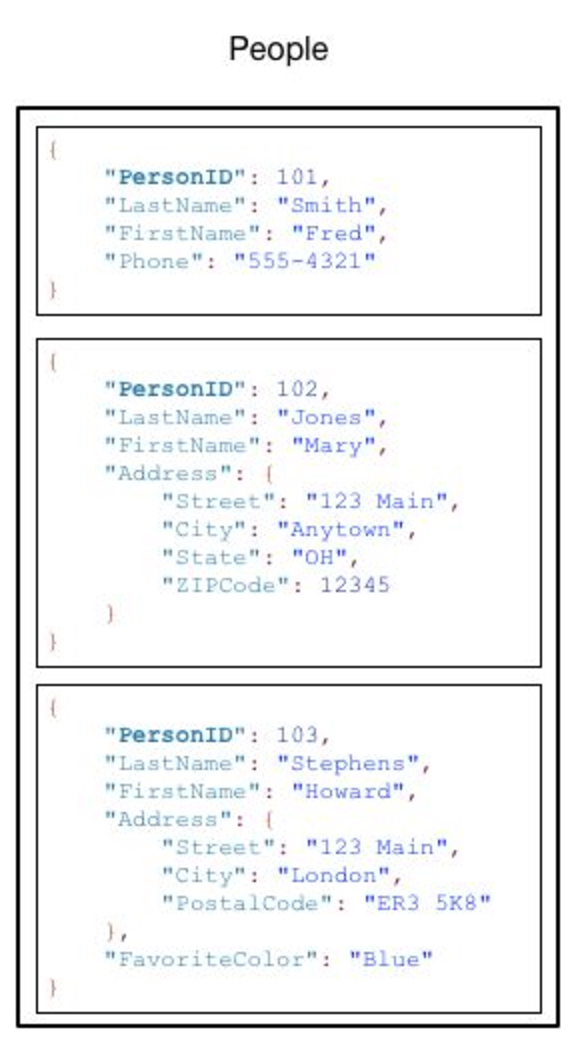
\includegraphics[width=0.3\textwidth]{images/dynamodb-basic-table.jpg}
\caption{This figure shows a table named \textit{People} with some example items and attributes. \cite{AmazonWebServices2013}}
\end{figure}

\subsection{Primary Key}
When creating a table a primary key \textbf{must} be specified. It uniquely identifies an item of a table, therefore it is not allowed that multiple items have the same primary key.
Each primary key attribute must be a scalar type. (See Section \ref{sssec:scalar}.)

\subsubsection{Partition key}
\label{sssec:partkey}
The \textbf{partition key} is a simple primary key composed of one attribute. DynamoDB will create a hash out of the key's value. This hash decides on which partition the item will be stored.

\subsubsection{Partition key and sort key}
In contrast to exclusive partition key (Section \ref{sssec:partkey}) it is possible that multiple items have the same primary key but must have a different sort key value. All items with the same partition key are stored together, in sorted order by the specified sort key value.

\subsubsection{Secondary Indexes}
A secondary index lets you query the data in the table using an alternate key, in addition to queries against the primary key. This can improve the performance of specific queries.
Indexes are maintained automatically during add, update or delete of an item. 


\subsubsection{DynamoDB Streams}

\subsection{Data Types}
DynamoDB offers a lot of different data types. These data types can be categorised as follows:

\begin{itemize}
    \item Scalar Types
    \item Document Types
    \item Set Types
\end{itemize}

\subsubsection{Scalar Types}
\label{sssec:scalar}
A scalar type can represent exactly one value. Possible scalar types are: \textbf{number}, \textbf{string}, \textbf{binary}, \textbf{boolean} and \textbf{null}.

\paragraph{Note:} DynamoDB does not offer a special data type for dates. To represent a date you either have to use a string (e.g. ISO 8601 string) or a number (e.g. epoch time).

\subsubsection{Document Types}
There are three document types: lists, maps and sets. These types can be nested within each other, to represent complex data structures up to 32 levels deep.

\paragraph{List}A list type attribute can store an ordered collection of values. A list is very similar to a JSON array.

\begin{lstlisting}[caption={Example of a DynamoDB list}, captionpos=b]
	Calculation: ["sum", "*", 4, "/", "3.939"]
\end{lstlisting}

\paragraph{Map}A map type attribute can store an unordered collection of key-value pairs. A map is very similar to a JSON object.
\begin{lstlisting}[caption={Example of a DynamoDB map}, captionpos=b]
	{
		User: "fahu",
		Date: "2017-06-28",
		VisistedWebsites: ["https://medium.com", "https://derstandard.at", "http://delta-xi.net/"]
	}
\end{lstlisting}

\paragraph{Sets}DynamoDB supports types that represent \textbf{sets} of \textbf{numbers}, \textbf{strings} and \textbf{binary} values. All elements of a set must be of the same data type. Each value within a set must be unique.

\begin{lstlisting}[caption={Example of a DynamoDB set}, captionpos=b]
	["black", "blue", "red, "green", "yellow"]
\end{lstlisting}











































































